% ════════════════════════════════════════════
% 模型求解（5.1.4）
% ════════════════════════════════════════════
\subsubsection{结果与解读}

基于上述框架，本节对 500 条帖子逐项统计。求解环境为 Python 3，使用 pandas 完成类型转换与分组统计，使用 SciPy 完成相关检验与分布计算，全部结果由同一份只读原始数据生成。

首先给出变量字典。由表\ref{tab:q1_dict}可知，8 个字段中 7 个为输入、1 个为输出；X2、X3、X7 为离散类别，X4、X5、X6 为周期性时间标记，X1 与 Y1 为连续数值。X1 只有 90 个不同取值且无缺失，说明粉丝数按天或按批次更新，同一数值被多条帖子共享；X7 是唯一存在缺失的字段。

\begin{longtable}{>{\centering\arraybackslash}p{0.08\textwidth}>{\centering\arraybackslash}p{0.21\textwidth}>{\centering\arraybackslash}p{0.11\textwidth}>{\centering\arraybackslash}p{0.12\textwidth}>{\centering\arraybackslash}p{0.20\textwidth}>{\centering\arraybackslash}p{0.08\textwidth}}
  \caption{变量字典}
  \label{tab:q1_dict} \\
  \toprule
  变量 & 含义 & 数据类型 & 因果角色 & 取值范围/类别 & 缺失 \\
  \midrule
  \endfirsthead
  \caption{变量字典（续）} \\
  \toprule
  变量 & 含义 & 数据类型 & 因果角色 & 取值范围/类别 & 缺失 \\
  \midrule
  \endhead
  \bottomrule
  \endfoot
  X1 & 粉丝规模（主页粉丝数） & 连续 & 状态/规模 & 81,370 至 139,441 & 0 \\
  X2 & 帖子类型（载体形式） & 名义 & 发帖决策 & Photo、Status、Link、Video & 0 \\
  X3 & 内容类别（内容主题） & 名义 & 发帖决策 & 1、2、3 & 0 \\
  X4 & 发帖月份 & 有序/周期 & 发帖决策 & 1 至 12 & 0 \\
  X5 & 发帖星期 & 有序/周期 & 发帖决策 & 1 至 7 & 0 \\
  X6 & 发帖时段（小时） & 有序/周期 & 发帖决策 & 0 至 23（样本 1 至 23） & 0 \\
  X7 & 是否付费推广 & 二元 & 发帖决策 & 0、1 & 1 \\
  Y1 & 曝光总次数 & 连续（计数） & 结果 & 570 至 1,110,282 & 0 \\
\end{longtable}

进一步给出描述性统计。表\ref{tab:q1_desc}显示，曝光量均值为 29,586 次，约为中位数 9,051 次的 3.27 倍，最大值 1,110,282 次为中位数的 122.67 倍，偏度 8.33、峰度 93.05，呈典型的重尾右偏形态。粉丝规模均值 123,194 人、标准差 16,273 人，最大值与最小值之比仅 1.71，量级跨度有限。付费帖子 139 条，占 499 条有效记录的 27.9\%（填补后占 500 条的 27.8\%），属于少数但不算稀疏的类别。

\begin{longtable}{>{\centering\arraybackslash}p{0.08\textwidth}>{\centering\arraybackslash}p{0.10\textwidth}>{\centering\arraybackslash}p{0.10\textwidth}>{\centering\arraybackslash}p{0.10\textwidth}>{\centering\arraybackslash}p{0.10\textwidth}>{\centering\arraybackslash}p{0.10\textwidth}>{\centering\arraybackslash}p{0.07\textwidth}>{\centering\arraybackslash}p{0.07\textwidth}}
  \caption{描述性统计}
  \label{tab:q1_desc} \\
  \toprule
  变量 & 均值 & 标准差 & 最小值 & 中位数 & 最大值 & 偏度 & 峰度 \\
  \midrule
  \endfirsthead
  \caption{描述性统计（续）} \\
  \toprule
  变量 & 均值 & 标准差 & 最小值 & 中位数 & 最大值 & 偏度 & 峰度 \\
  \midrule
  \endhead
  \bottomrule
  \endfoot
  X1 & 123194 & 16273 & 81370 & 129600 & 139441 & $-0.980$ & $-0.276$ \\
  X3 & 1.880 & 0.853 & 1 & 2 & 3 & 0.231 & $-1.584$ \\
  X4 & 7.038 & 3.308 & 1 & 7 & 12 & $-0.122$ & $-1.137$ \\
  X5 & 4.150 & 2.031 & 1 & 4 & 7 & $-0.102$ & $-1.275$ \\
  X6 & 7.840 & 4.369 & 1 & 9 & 23 & 0.213 & $-0.825$ \\
  X7 & 0.279 & 0.449 & 0 & 0 & 1 & 0.988 & $-1.024$ \\
  Y1 & 29586 & 76803 & 570 & 9051 & 1110282 & 8.326 & 93.053 \\
  logY & 9.381 & 1.178 & 6.347 & 9.111 & 13.920 & 0.734 & 0.821 \\
\end{longtable}

表\ref{tab:q1_collin}把尾部与共线证据集中列出。变换后曝光量偏度降至 0.734、峰度降至 0.821，说明 log1p 能有效压缩尾部。粉丝规模与月份的 Pearson 相关为 0.941、Spearman 相关为 0.996，月份哑变量对粉丝规模对数的解释度达 0.9917，月内标准差仅 0.0130、方差占比仅 0.83\%。按上述判别准则，四项条件同时满足，粉丝规模与月份属于同一变异维度。

\begin{longtable}{>{\centering\arraybackslash}p{0.34\textwidth}>{\centering\arraybackslash}p{0.14\textwidth}>{\centering\arraybackslash}p{0.44\textwidth}}
  \caption{共线与分布指标}
  \label{tab:q1_collin} \\
  \toprule
  指标 & 数值 & 说明 \\
  \midrule
  \endfirsthead
  \caption{共线与分布指标（续）} \\
  \toprule
  指标 & 数值 & 说明 \\
  \midrule
  \endhead
  \bottomrule
  \endfoot
  样本量 & 500 & 每条记录对应一条帖子 \\
  变量数 & 8 & 7 个输入加 1 个输出 \\
  完全重复行 & 0 & 按 8 个原始变量判定 \\
  X7 缺失数 & 1 & 占 0.2\%，仅第 499 行缺失 \\
  Y1 偏度（原始） & 8.326 & 右偏严重 \\
  Y1 峰度（原始） & 93.053 & 超额峰度，尾部极厚 \\
  Y1 最大值/中位数 & 122.67 & 极端值相对规模 \\
  log1p(Y1) 偏度 & 0.734 & 变换后接近对称 \\
  log1p(Y1) 峰度 & 0.821 & 峰度显著下降 \\
  Pearson $r(X_1,X_4)$ & 0.941 & 线性同步程度高 \\
  Spearman $\rho(X_1,X_4)$ & 0.996 & 单调同步程度极高 \\
  $R^2(\log X_1\sim\text{月份})$ & 0.9917 & 99.17\% 的变异在月间 \\
  月内 $\log X_1$ 标准差 & 0.0130 & 总标准差为 0.1435 \\
  月内方差占比 & 0.0083 & 月内仅剩 0.83\% 的信息 \\
\end{longtable}

如图\ref{fig:q1_dist}所示，曝光量分布跨越三个数量级，直方图在对数横轴上仍呈明显右偏，中位数附近堆积了大量帖子，而 10 万次以上的极端帖子数量很少。分组箱线图显示，付费组的中位曝光为 12,060 次，高于自然组的 8,387 次；视频组与状态组的中位数整体高于图片组，链接组与图片组接近。这些差异为后续回归提供了初步线索，但分组比较未控制月份与主题，不能直接当作净效应。

\begin{figure}[ht]
  \centering
  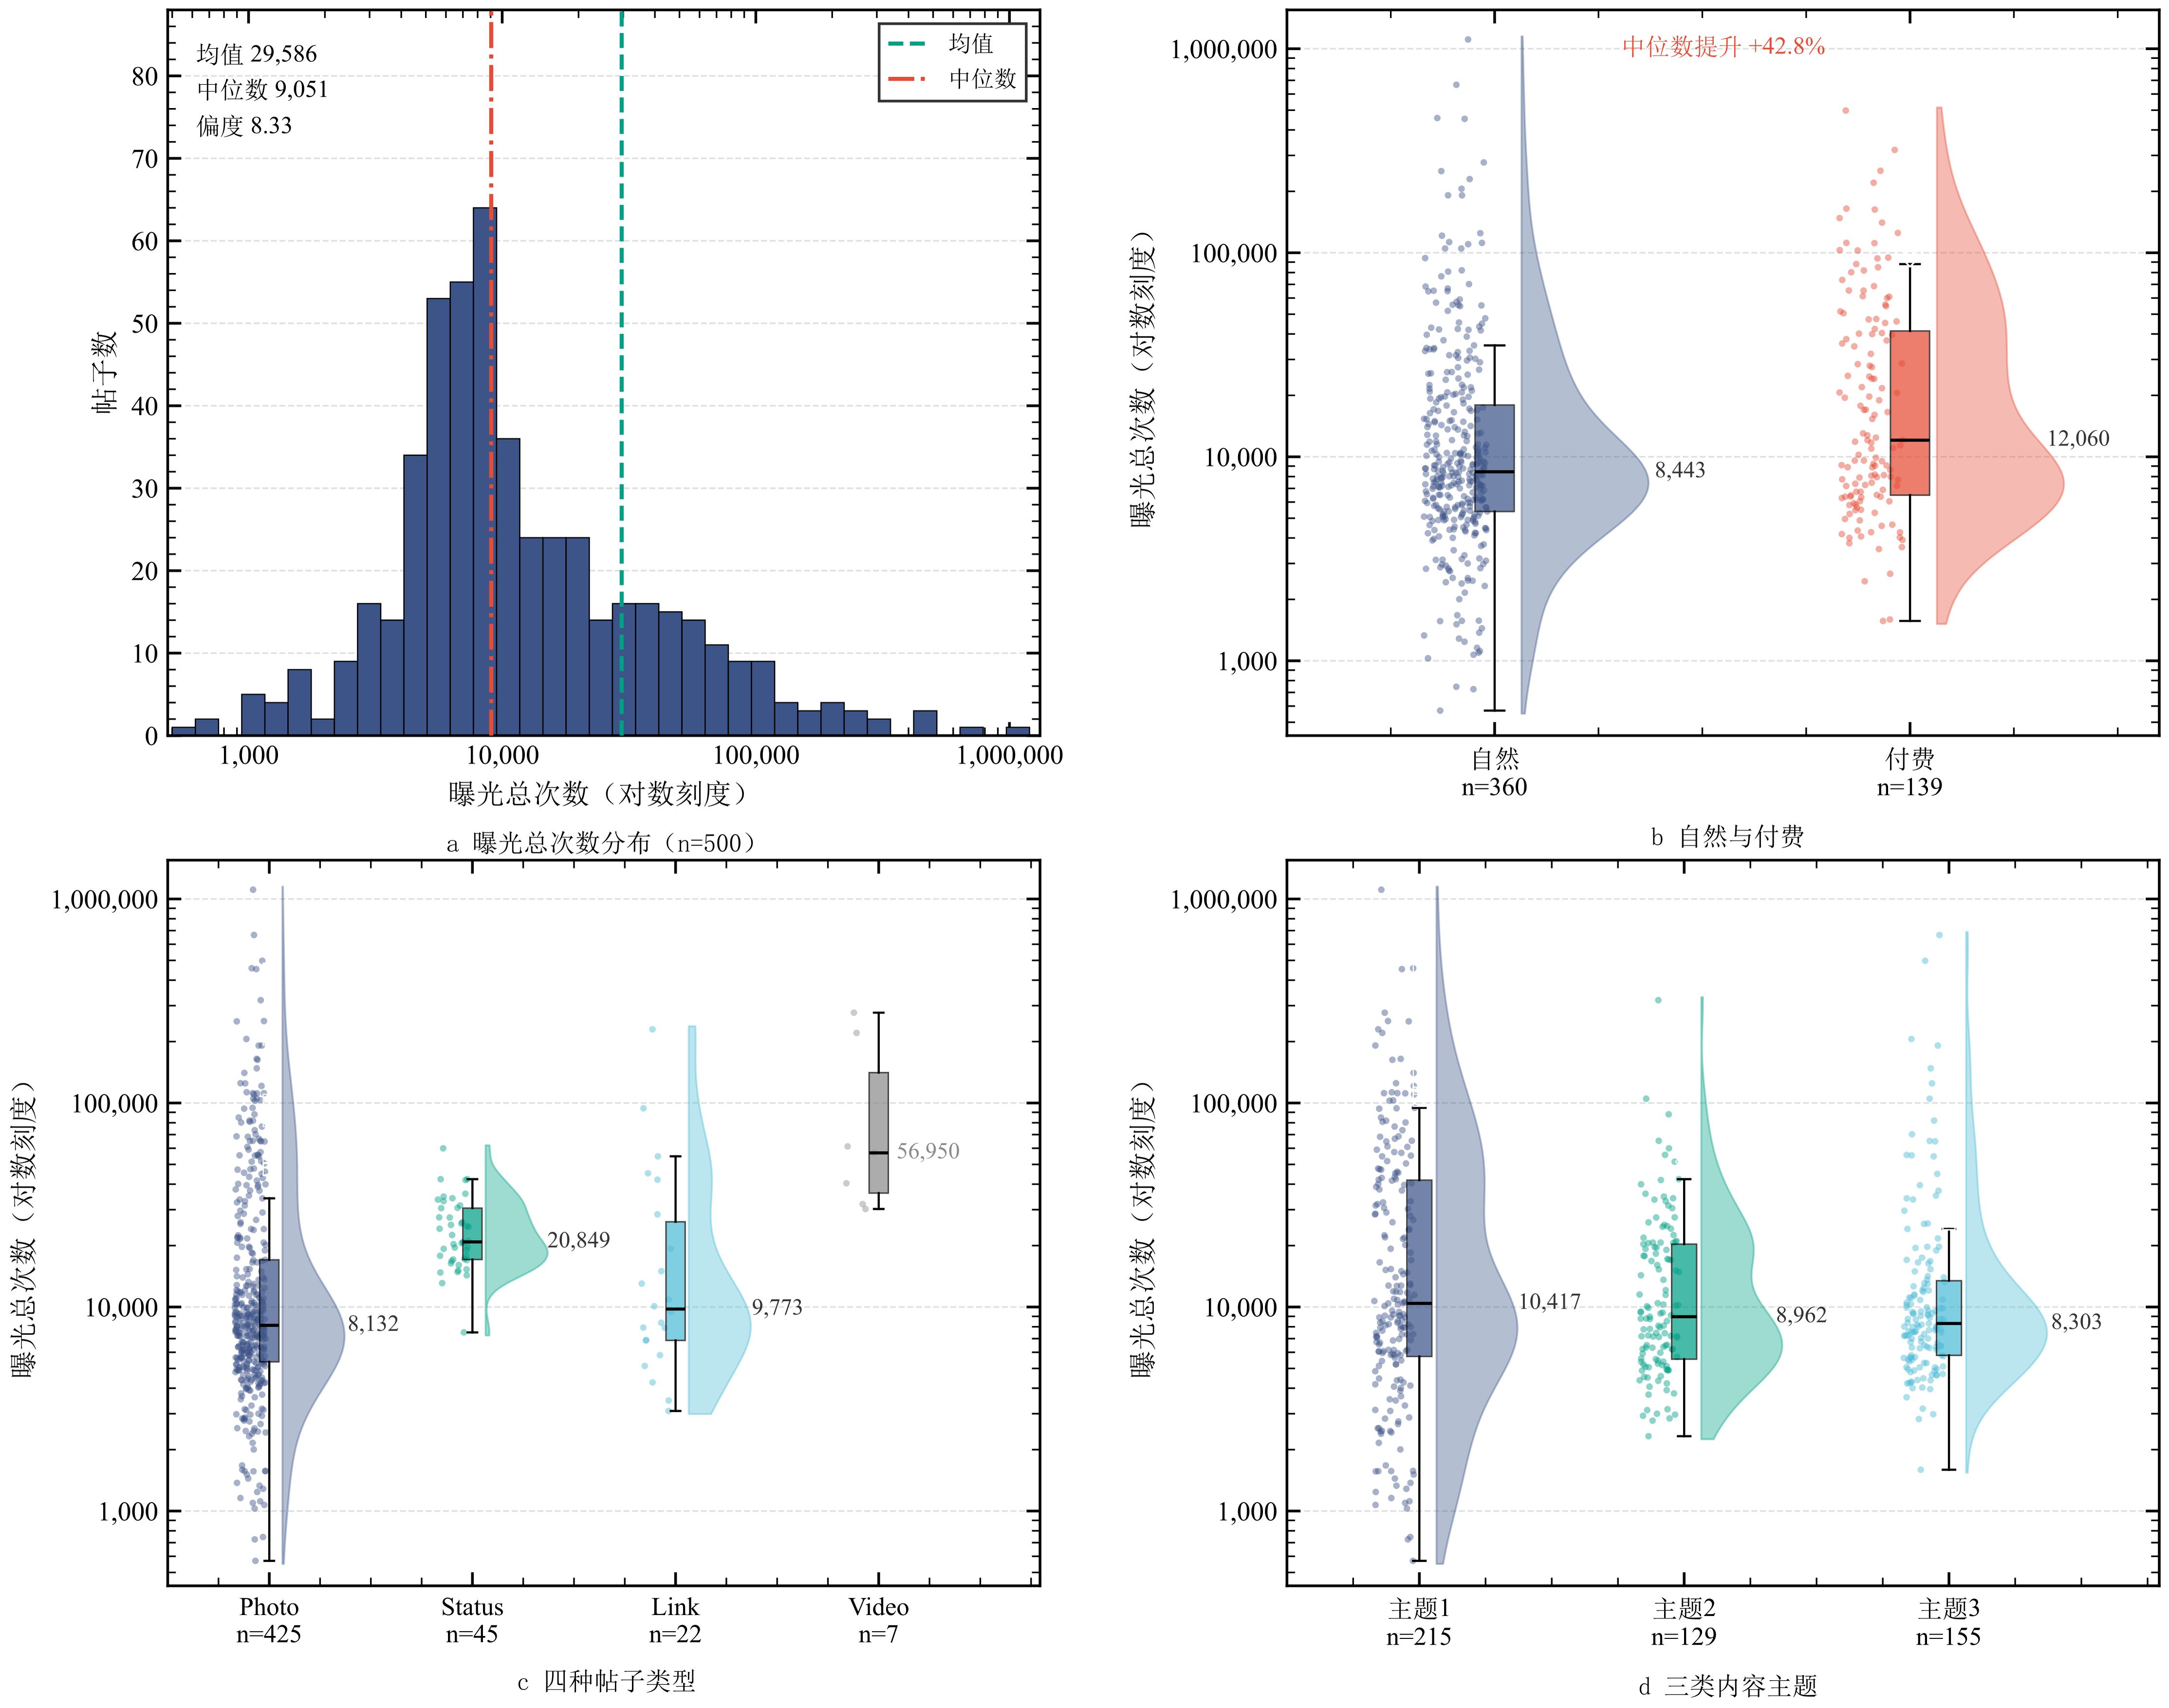
\includegraphics[width=0.68\textwidth]{../求解/问题一/结果/图1_曝光与分组分布.png}
  \caption{曝光量分布与分组差异}
  \label{fig:q1_dist}
\end{figure}

图\ref{fig:q1_structure}从构成、主题分布与联合分布三个角度补充样本结构。左上图以中线为界，左侧为自然帖、右侧为付费帖：Photo 在两组中都占 85\% 以上，Status 与 Link 合计不足 15\%，Video 只有 7 条且其中 4 条为付费，说明类型效应主要由 Photo 与 Status 支撑，Video 的估计必然带有较大不确定性。右上图把三类主题的曝光分布、箱线与原始散点叠在一起，三组对数曝光的中位数分别为 9.25、9.09、9.02，主题1 的分布整体略高，但三组重叠很大，单看主题不足以区分帖子表现。下方联合密度图的散点呈近竖直云团，粉丝规模对数与曝光对数的 Pearson 相关系数仅为 $-0.082$（$p=0.066$），上缘与右缘的边缘直方图进一步显示：两组在粉丝规模上几乎完全重合，而在曝光轴上付费组整体右移。由此可见，粉丝规模既不能单独解释曝光，也不足以区分付费与自然帖子，后续模型应把重点放在内容与投放变量上。

\begin{figure}[ht]
  \centering
  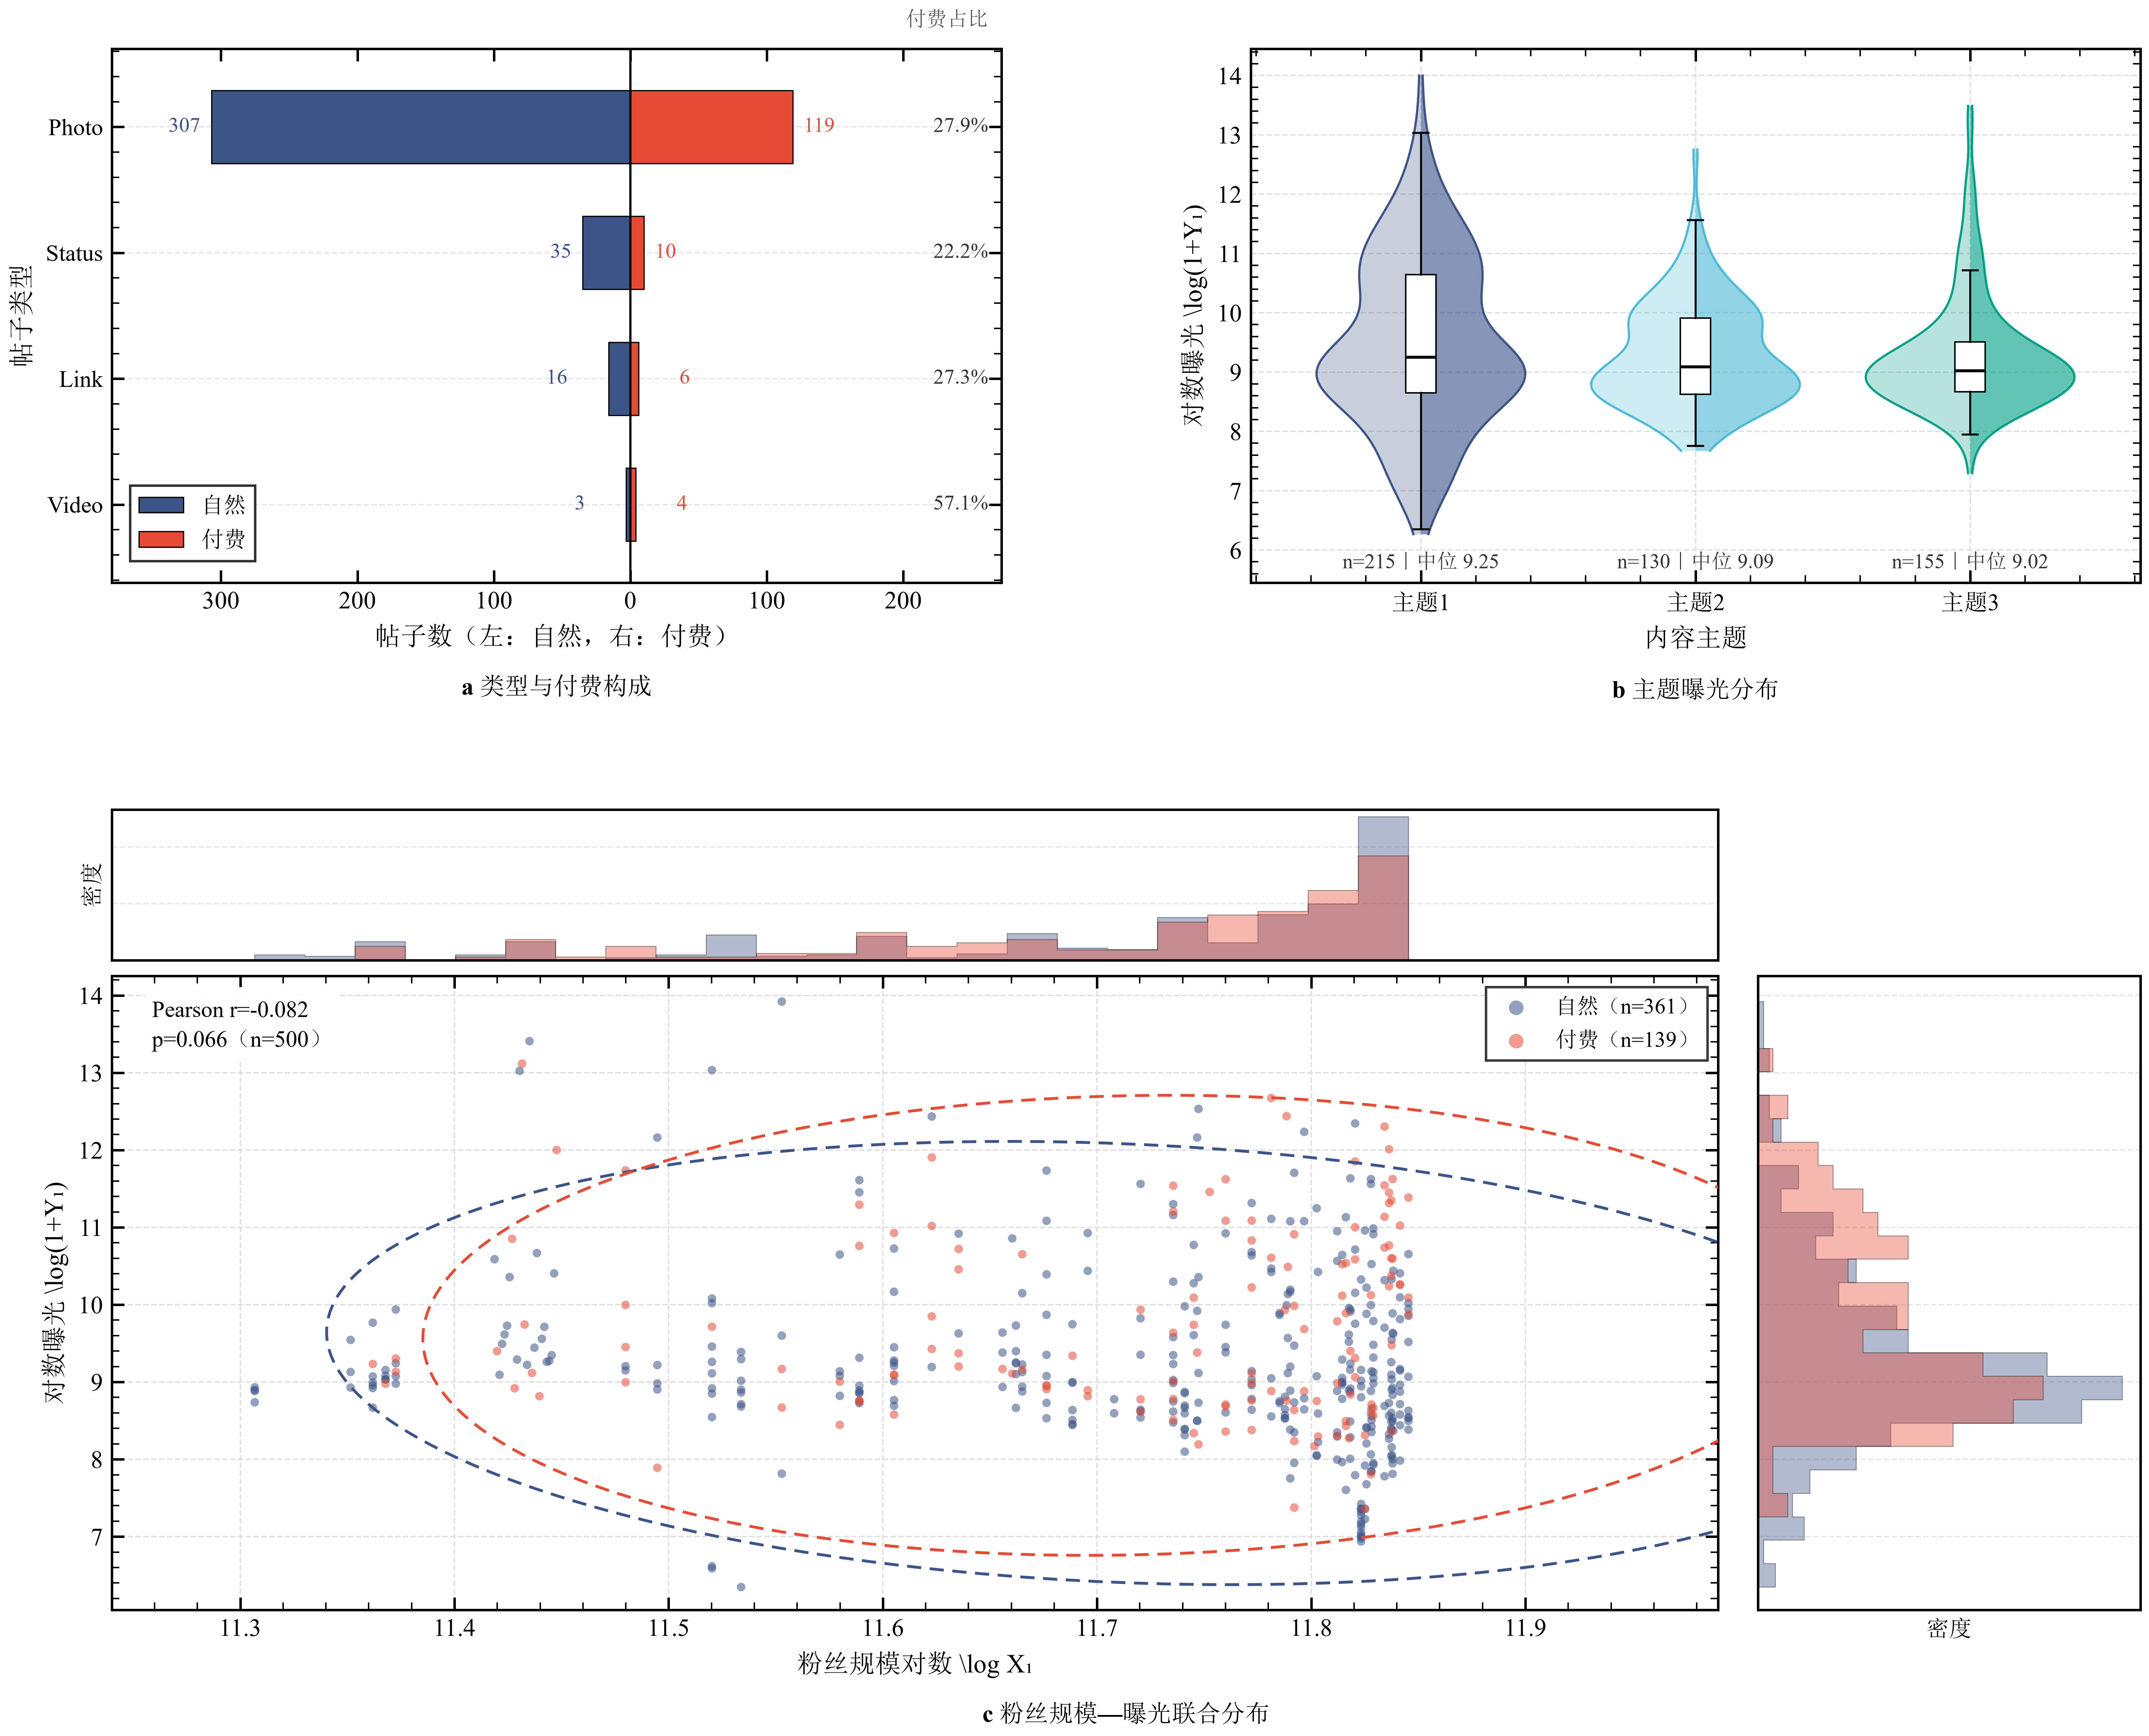
\includegraphics[width=0.82\textwidth]{../求解/临时产物/补充图1_样本结构.png}
  \caption{样本构成、主题分布与粉丝—曝光联合分布}
  \label{fig:q1_structure}
\end{figure}

图\ref{fig:q1_month}进一步展示了核心共线结构。散点沿月份呈阶梯式上升，月均值折线几乎单调递增；下方月内偏差小图显示，同一月份内部的粉丝规模对数只在极小范围内波动，偏差幅度远小于月间差异。这说明粉丝规模在本样本中更接近“时间标签”而非独立解释变量，若把它与月份同时放入回归，月份哑变量与粉丝规模会互相吸收，系数估计将依赖极少量月内变异。

\begin{figure}[ht]
  \centering
  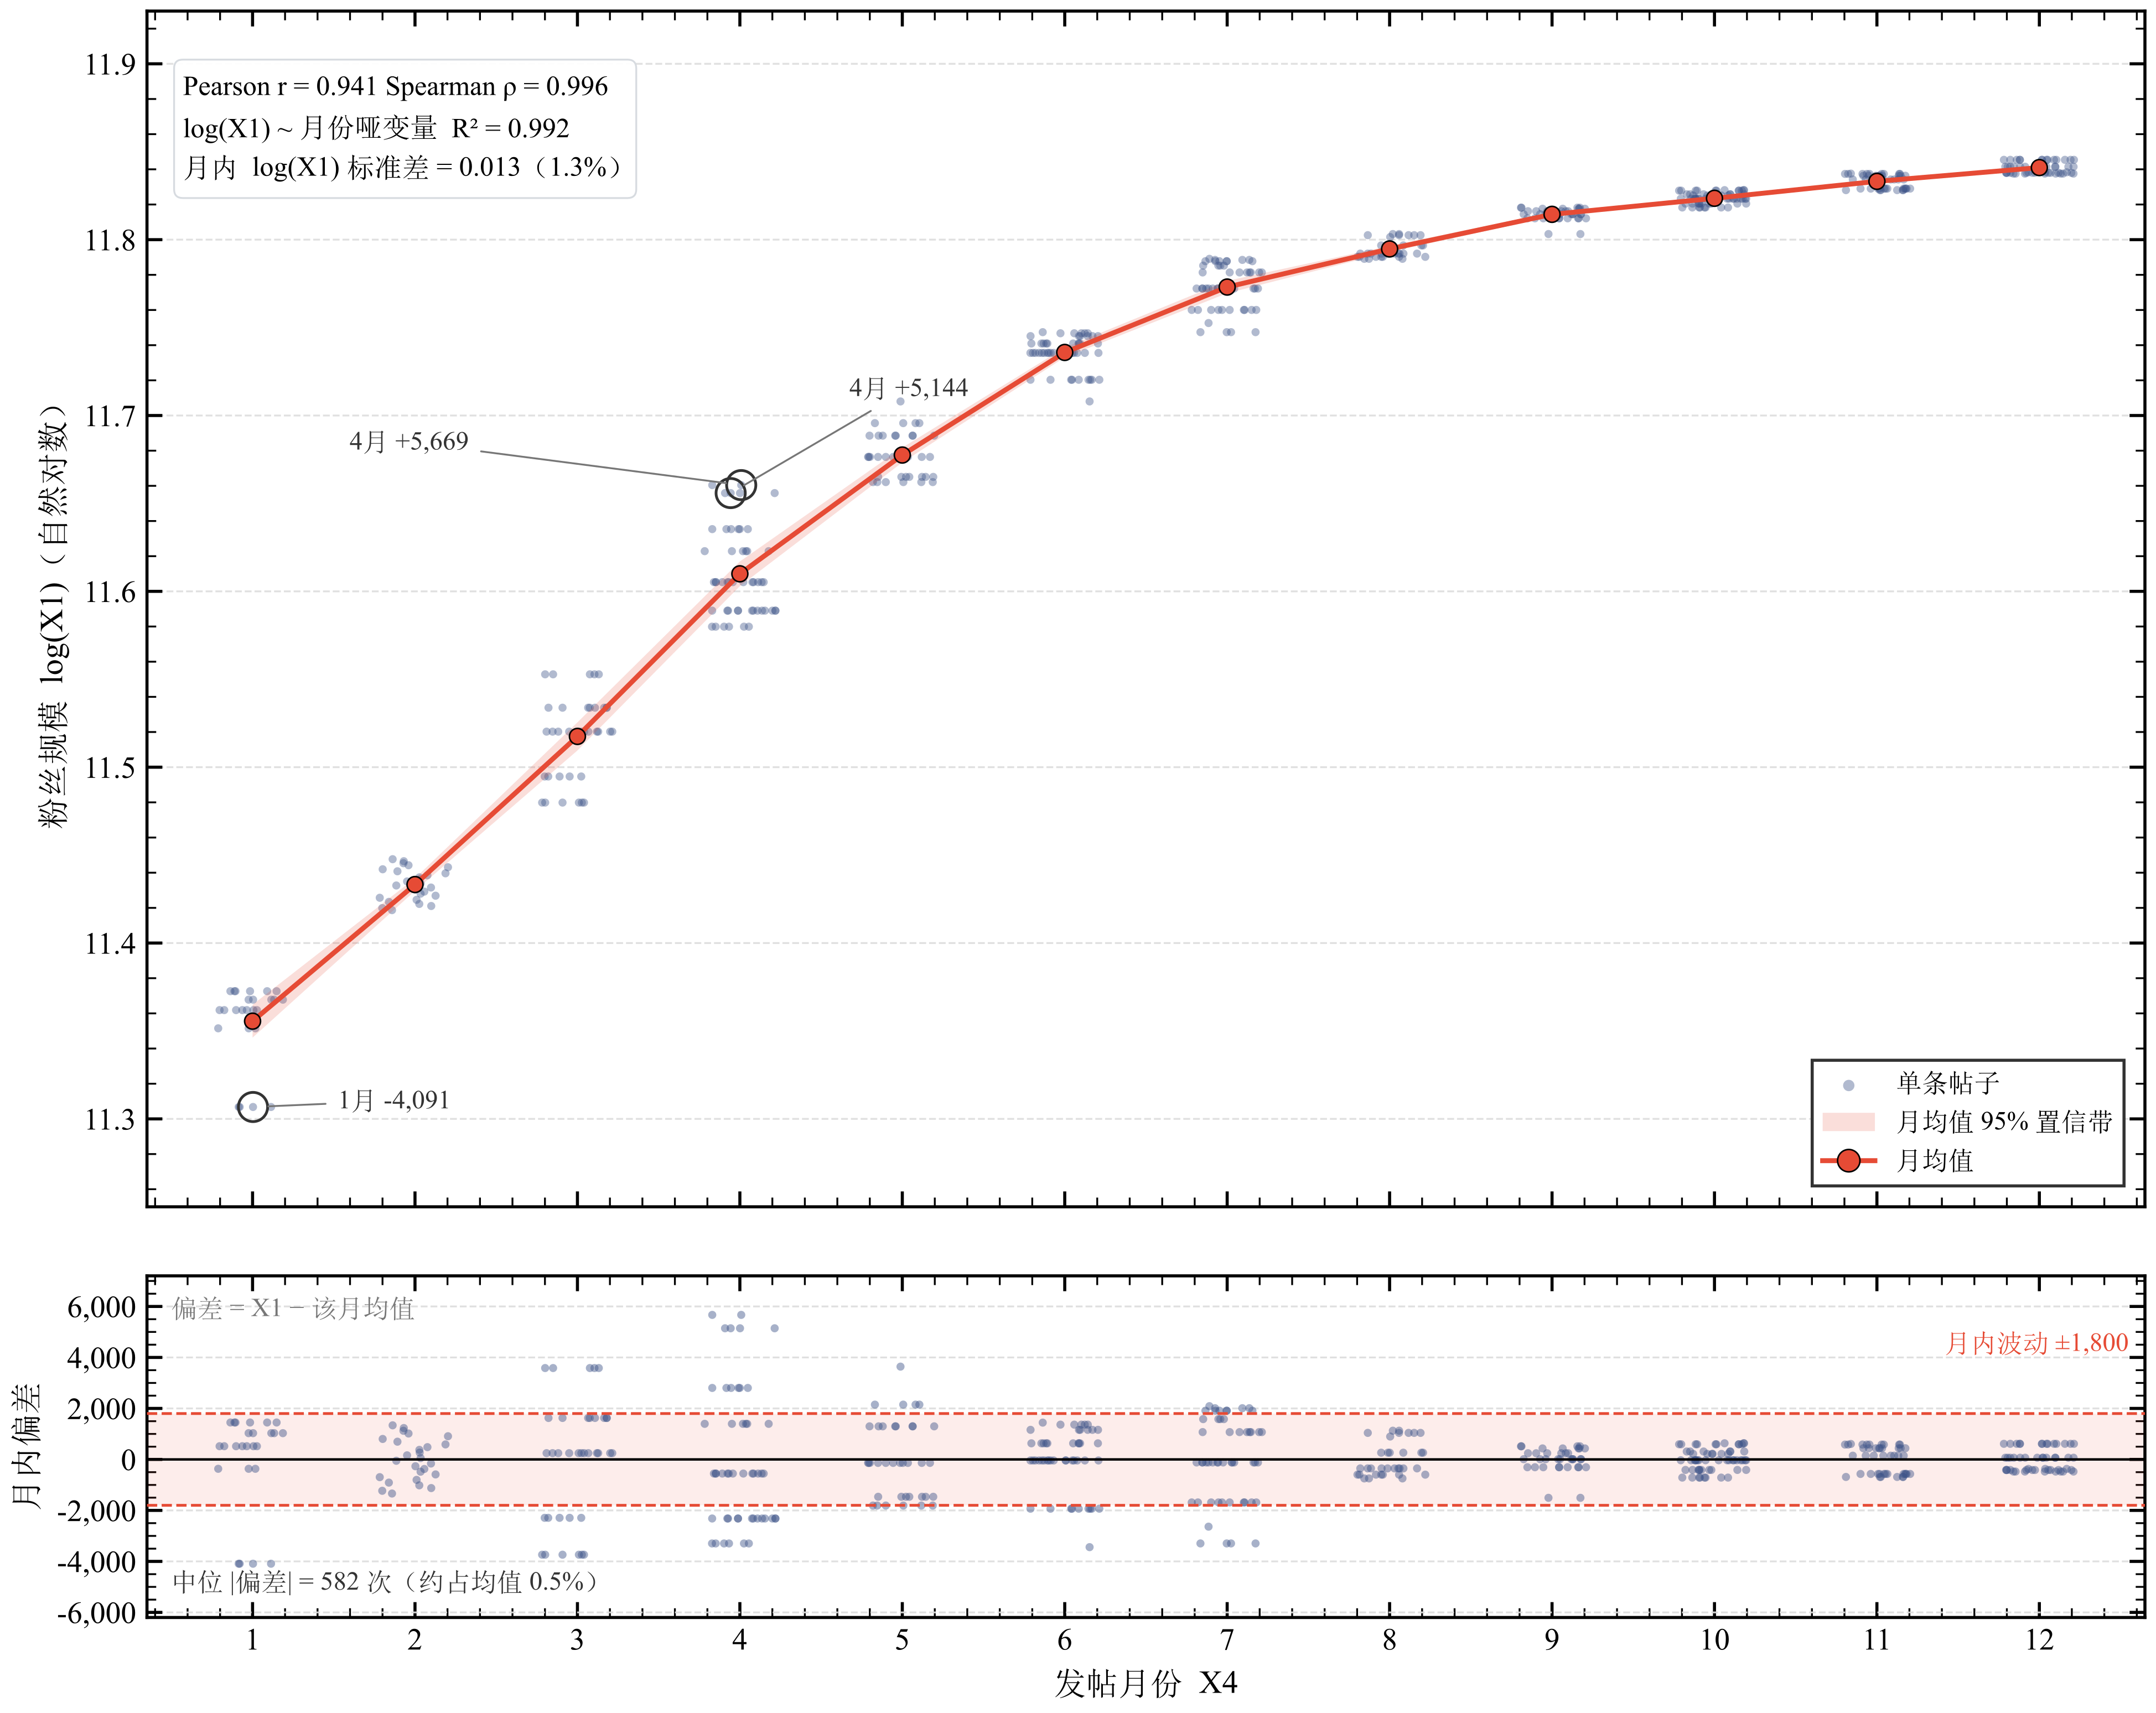
\includegraphics[width=0.75\textwidth]{../求解/问题一/结果/图2_粉丝规模与月份共线.png}
  \caption{粉丝规模与月份的共线结构}
  \label{fig:q1_month}
\end{figure}

图\ref{fig:q1_corr}给出主要变量的 Spearman 相关矩阵。曝光量与付费的相关系数为 0.171，是矩阵中与曝光关系最强的一项；与粉丝规模、月份的相关系数均为 $-0.135$，与内容主题为 $-0.080$，方向虽为负但幅度都很小。粉丝规模与月份的相关系数为 0.996，是矩阵中最突出的一格，说明二者几乎携带同一信息。相关矩阵只反映两两关系，且不包含帖子类型与发布时段，仍需回归控制其他变量后才能判断净效应。

\begin{figure}[ht]
  \centering
  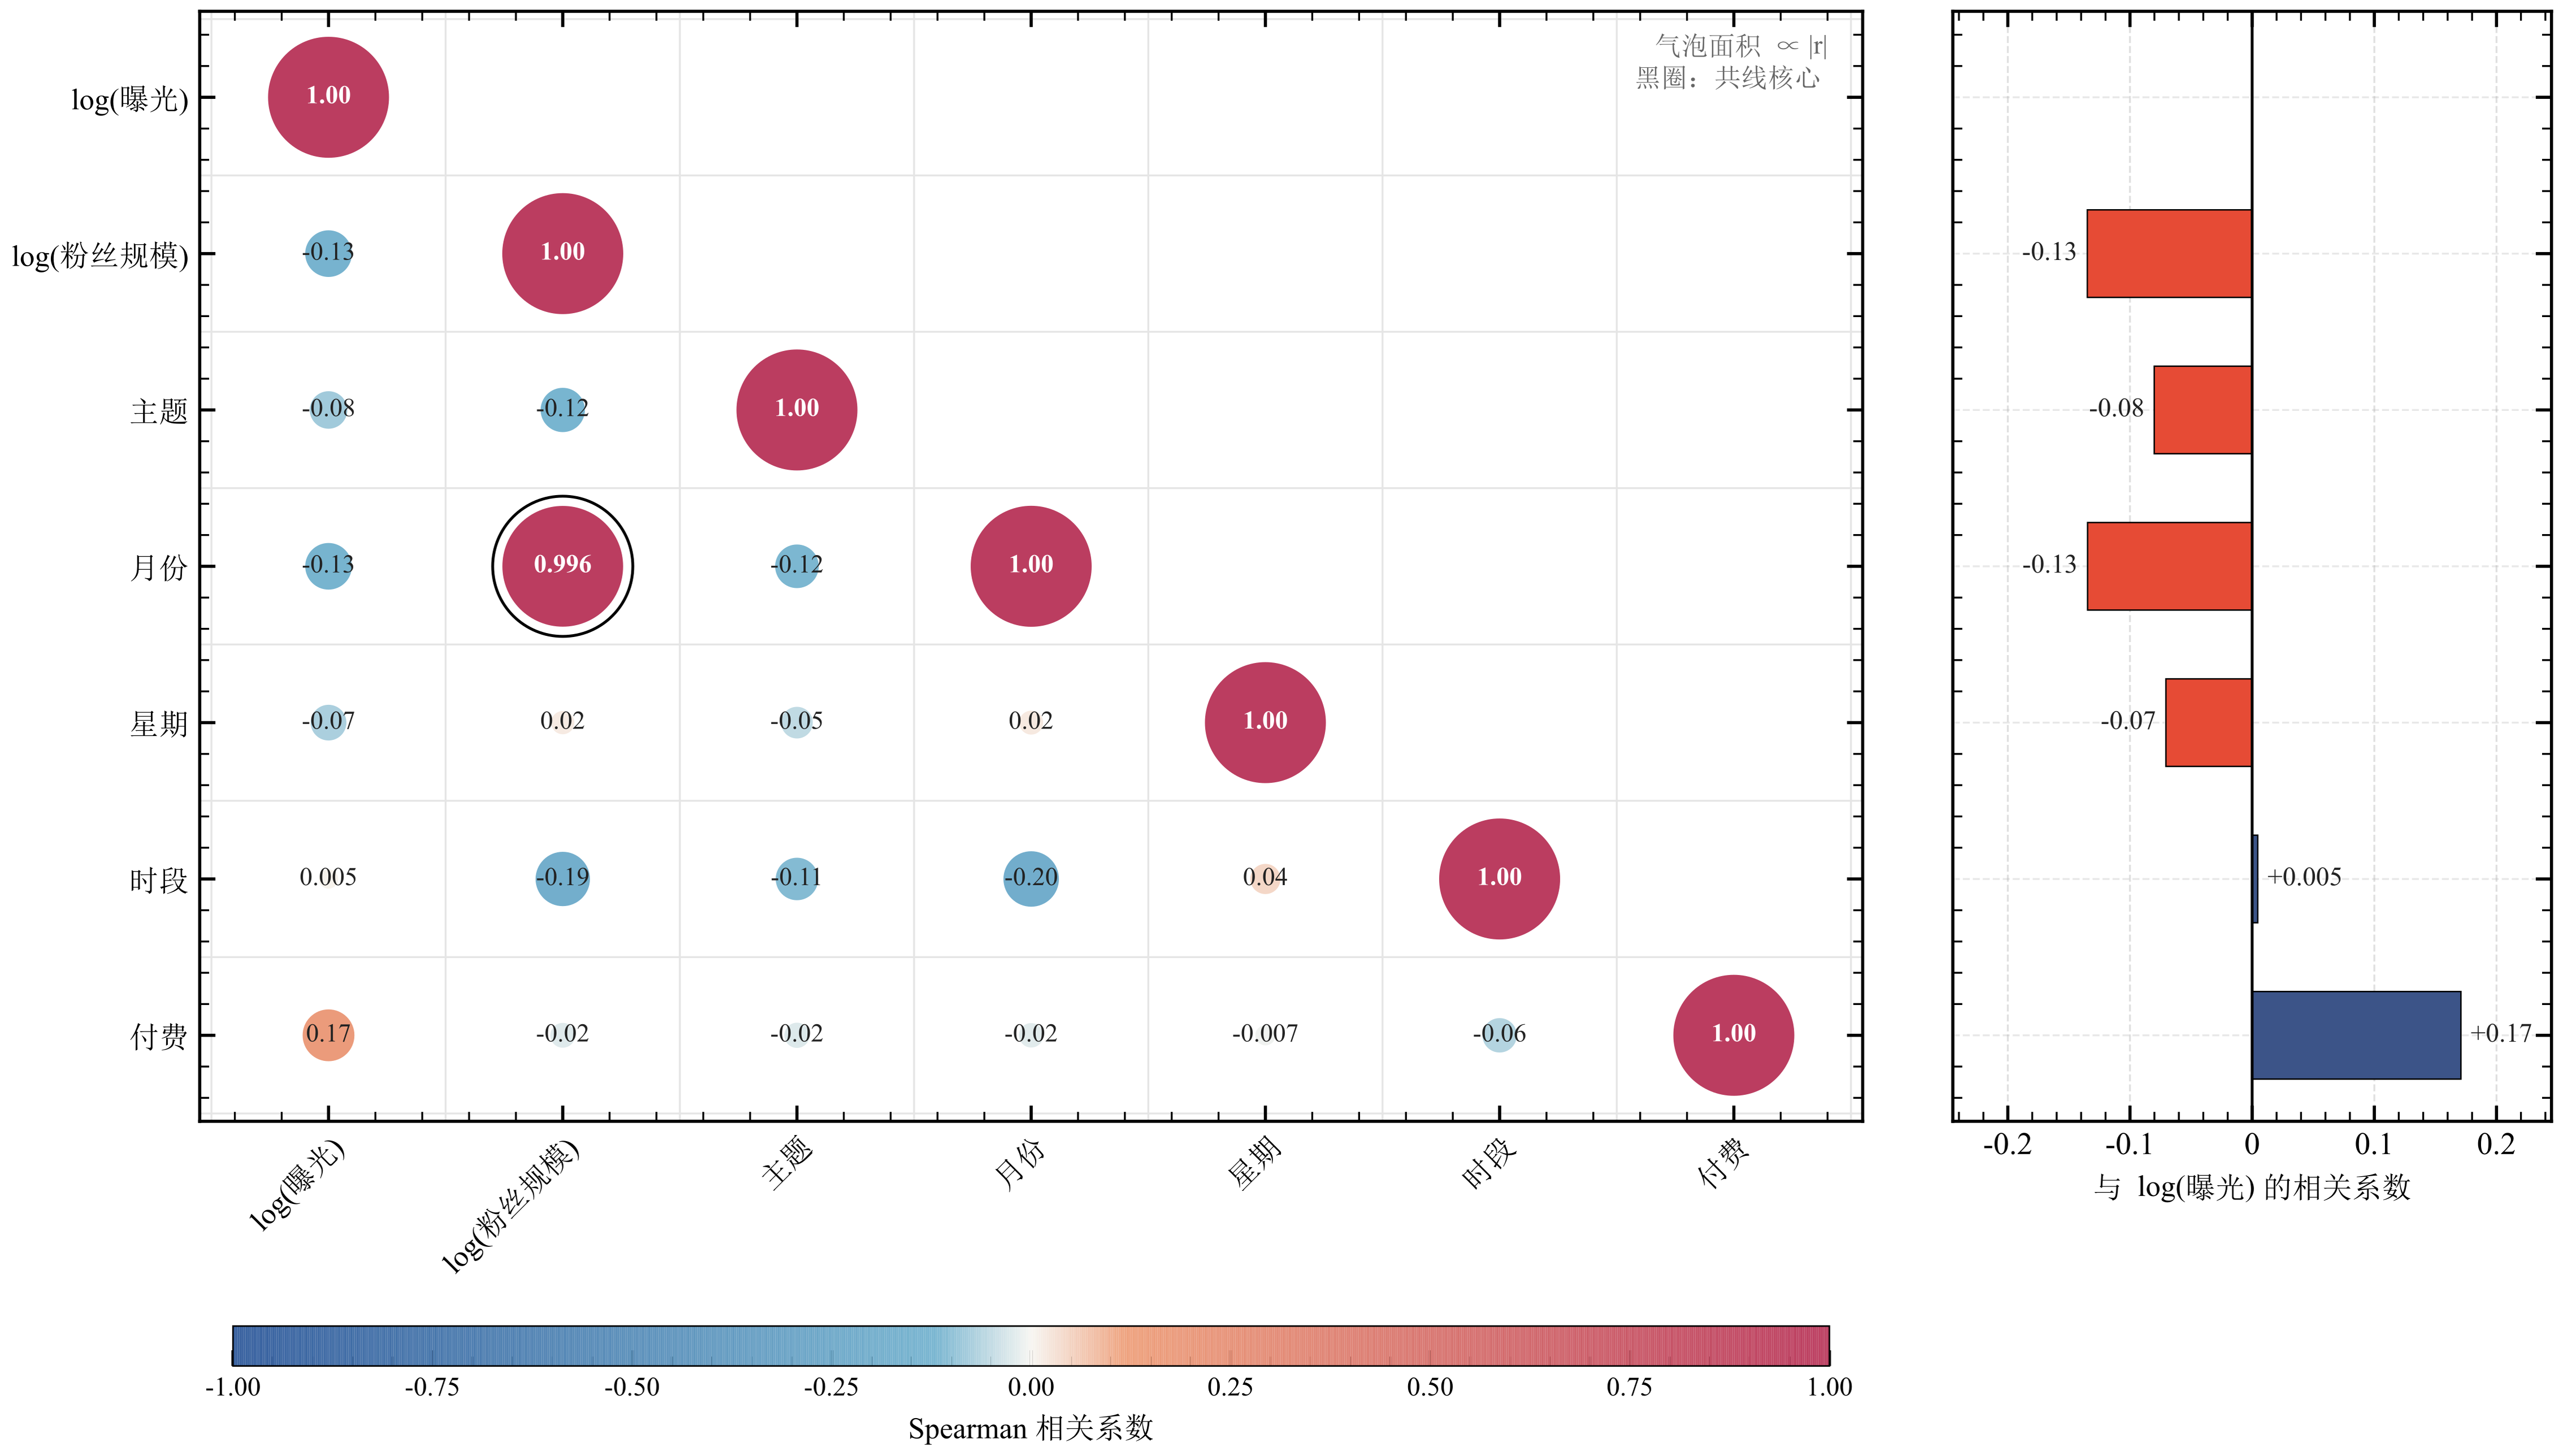
\includegraphics[width=0.66\textwidth]{../求解/问题一/结果/图3_相关系数热力图.png}
  \caption{主要变量的 Spearman 相关系数}
  \label{fig:q1_corr}
\end{figure}

综合以上结果，500 条帖子构成一份帖子级截面数据，曝光量重尾、类别不平衡、粉丝规模与月份近乎共线。数据理解的核心结论不是“粉丝规模影响曝光”，而是“粉丝规模与月份共同刻画了账号成长的时间维度，二者不能同时识别”。这一结论直接决定了后续的建模策略：以月份固定效应吸收规模趋势，把粉丝规模留作稳健性对照，而不是强行解释其系数。
